\documentclass[english]{panikzettel}

\usepackage{listings}
\lstset{escapechar=\&,
        stringstyle=\ttfamily,
        keywordstyle=\bold,
        emph={Action, Precond, Effect, Op},
        emphstyle={\bfseries}
    }

\usepackage{nicefrac}

\title{Introduction to Artificial Intelligence Panikzettel}
\author{Philipp Schröer, Der Dude, Luca Oeljeklaus}

\begin{document}

\maketitle

\tableofcontents

\section{Introduction}

This Panikzettel is about the lecture Introduction to Artificial Intelligence by Prof.\ Lakemeyer held in the winter semester 2017/18.

This Panikzettel is Open Source. We appreciate comments and suggestions at \\ \url{https://git.rwth-aachen.de/philipp.schroer/panikzettel}.

\section{Agent Architectures}

\subsection{Agent Types}

An \emph{agent} has \emph{effectors} to influence its environment, based on \emph{percepts} that are perceived  through the agent's \emph{sensors}.
A \emph{rational agent} acts according to some performance criteria.
Rational action depends on the performance measure, the percept sequence, world knowledge and possible actions.

If you're the acronym type, you can remember this as \emph{PAGE}: \emph{percepts}, \emph{actions}, \emph{goals}, \emph{environment}.

A \emph{table-lookup agent} has a mapping indexed by percept sequences.
Each action is just an entry in that table.

A \emph{reflexive agent} has a set of condition-action rules that are pattern matched against a percept.
Additionally, a \emph{reflexive agent with an internal world model} may have a state machine as memory.

\emph{Goal-oriented agents} try to fulfil (binary) goals by imagining the outcome of actions.
\emph{Utility-based agents} have a utility function that judges the expected outcomes of different actions somehow.
This allows more flexibility, especially with uncertainty or conflicting goals.

\emph{Learning agents} have a \emph{learning element} that improves the system by changing and retrieving knowledge from the \emph{performance element} (agent in the old sense, handles effectors).
The \emph{critic} judges sensor data and gives feedback to the learning element.
Additionally, there's a \emph{problem generator} that suggests actions to test performance of the performance element.

\newpage
\subsection{Environment Properties}

\begin{itemize}
    \item \emph{accessible} (as opposed to \emph{nonaccessible}): \\
          All relevant aspects of the world are available to the sensors.
    \item \emph{deterministic} (as opposed to \emph{nondeterministic}/\emph{stochastic}): \\
          The next state depends completely on the current state and chosen action.
    \item \emph{episodic} (as opposed to \emph{nonepisodic}): \\
          The choice of an action depends only on the current state (not on the past).
    \item \emph{static} (as opposed to \emph{dynamic}): \\
          The world does not change while deciding on an action.
    \item \emph{discrete} (as opposed to \emph{continuous}): \\
          There are only finitely many world states in a range.
\end{itemize}

\section{Search}

\subsection{Search Problems}

\begin{halfboxl}
This section is concerned with goal-oriented agents.
Given an \emph{initial state} of the world, an agent searches through a \emph{state space}, where world states are connected by actions of the agent.
The agent tries to find a sequence of actions leading to a world state that satisfies a goal (\emph{goal test}).

The connections of states are given by the \emph{operator}: It gives a description of which state is reached by an action from a given state. The \emph{successor function} $S(x)$ returns the set of states reachable by any action from state $x$.

A sequence of actions is called a \emph{path}.
Paths have a \emph{past cost}.
A \emph{solution} is a path from the initial state to a state that satisifies the goal test.

Finding a solution may have a \emph{search cost}.
The \emph{total cost} also includes the path cost to the solution.
\end{halfboxl}%
\begin{halfboxr}
\vspace{-\baselineskip}
\begin{defi}{State space}
\begin{itemize}
    \item Set of states
    \item Set of operators
    \item Goal test function
    \item Path cost function
    \item Search cost function
\end{itemize}
\end{defi}

\begin{defi}{Search problem}
Starting at an \emph{initial state}, search the state space to find a path to a goal state.

States are \emph{expanded} during search to create successor states.
This search induces a \emph{search tree}.
\end{defi}
\end{halfboxr}

There are varying degrees of difficulty for state space search problems.
\begin{center}
    \begin{tabular}{c|c|c}
        & World knowledge & Action knowledge \\ \hline
        \emph{Single-state problem} & complete & complete \\
        \emph{Multiple-state problem} & incomplete & complete \\
        \emph{Contingency problem} & to be found at run-time & incomplete \\
        \emph{Exploration problem} & unknown & unknown
    \end{tabular}
\end{center}

\newpage
\subsection{Search Strategies}

Search strategies can be evaluated by a few metrics:
\begin{itemize}
    \item \emph{Completeness}: Always finds a solution if it exists.
    \item \emph{Time complexity}: Worst case search time.
    \item \emph{Space complexity}: Worst case memory usage.
    \item \emph{Optimality}: Always finds the best solution, not just a solution.
\end{itemize}

An \emph{uninformed (blind) search} does not use any information about the length or cost of a solution.
An \emph{informed (heuristic) search} does have some information.

In the following, $b$ will be the maximum branching factor and $d$ the depth of a solution.

\subsubsection{Uninformed Search Strategies}

\emph{Breadth-first search (BFS)} expands nodes in the order they are generated.

\emph{Uniform cost search} is a modified BFS that expands nodes with the least path cost first.

\emph{Depth-first search (DFS)} always expands the node at the deepest level.

\emph{Depth-limited search} is a DFS that only expands up to a specified depth.

\emph{Iterative deepening} combines BFS and DFS. It executes depth-limited search at increasing depths until a solution is found.

If forward and backward searches are symmetric, then \emph{bidirectional search} is possible.

\begin{center}
    \footnotesize
    \begin{tabular}{c|c|c|c|c|c|c}
         Criterion & BFS & Uniform-Cost & DFS & Depth-Limited & Iterative Deepening & Bidirectional \\
         \hline
         Complete? & Yes & Yes & Yes & No & Yes & Yes\\
         Time & $\mathcal{O} (b^{d+1})$ & $\mathcal O(b^{1+\lfloor \nicefrac{C^\star}{\varepsilon}\rfloor}$ & $\mathcal O(b^m)$ & $\mathcal O(b^\ell)$ & $\mathcal O(b^d)$ & $\mathcal O(b^{\nicefrac d2})$\\
         Space & $\mathcal O(b^{d+1})$ & $\mathcal O(b^{1+\lfloor \nicefrac{C^\star}{\varepsilon}\rfloor}$ & $\mathcal O(bm)$ & $\mathcal O(b\ell)$ & $\mathcal O(bd)$ & $\mathcal O(b^{\nicefrac d2})$\\
         Optimal? & No & Yes (pos. costs) & No & No & No & No\\
    \end{tabular}
\end{center}

These properties hold with regard to finite graph assuming the algorithm tests for cycles and with $b$ being the maximal branching factor, $d$ the minimal depth of a goal state, $m$ the maximal search depth, $\ell$ the depth restriction, $C^\star$ the cost of the optimal path and $\varepsilon$ the minimum step cost.

\subsubsection{Informed Search Strategies}

\emph{Informed search strategies} use an \emph{evaluation function} $f$ that returns the cost to the goal from a given node.

\emph{Best-first Search} always expands the node with the best $f$-value.

\emph{Greedy search} always chooses the node with the minimal (expected) cost to the goal state.

\emph{$A^\ast$ search } combines uniform cost search with greedy search.
\begin{itemize}
    \item $g(n) = $ actual cost from initial state to $n$.
    \item $h(n) = $ estimated cost from $n$ to the nearest goal.
    \item $f(n) = g(n) + h(n)$, the estimated cost of the cheapest path through $n$.
\end{itemize}
The heuristic $h$ used for $A^\ast$ must be \emph{admissible}, that is $h(n) \leq h^\ast(n)$ must hold where $h^\ast (n)$ is the cost of an optimal path from $n$ to the nearest goal.

To compare the quality of admissible heuristics we introduce the effective branching factor $b^\ast$. If an instance of $A^\ast$ generates $N$ nodes and the solution depth is $d$ then $b^\ast$ is the solution of:

\[N+1 = 1 + \left(b^\ast \right)^1  + \dots + \left(b^\ast\right)^d\]

E.g.\ a tree of depth $d$ and branching factor $b^\ast$ would contain the same number of nodes as the tree generated during the search.

\emph{Iterative Deepening $A^\ast$} is a variant of Iterative Deepening search that explores branches up to a given threshold for the value of $f(n)$. If this threshold is passed and no solution was found the threshold is set to the minimal value of $f(n)$ for all found nodes $n$ that exceeded the threshold.

\emph{Simplified Memory-Bounded $A^\ast$} uses a bounded priority queue. New nodes are added to the queue.
Each time a node is added, the algorithm checks whether all sibling nodes are in the queue, then the parent is removed.
If the memory is full, the node with the highest cost is removed from the queue and its parent is added (if not already present).

\emph{Hill Climbing} simply iteratively expands the highest-valued successor of the current node.

\emph{Simulated Annealing} uses a \emph{temperature} that decreases with time. In each iteration, a random successor is chosen.
If the successor has a higher value, then the next iteration starts with this node, otherwise only with probability $e^{\Delta E / T}$ where $\Delta E$ is the value difference and $T$ is the temperature (iteration count).
Otherwise the iteration restarts with the old node.

\newpage
\section{Games}

\emph{Games} are special cases of search problems.
States are usually accessible.
\emph{Actions} are possible moves by a player.

From a player's point of view, there may be uncertain outcomes of actions, so games are contingency problems.

We will look at 2-person games.
The players are called MIN and MAX.
MAX moves first.
Operators are legal moves.

MAX needs to find a path which leads to a winning state for every possible reaction of MIN.

\begin{algo}{Minimax}
\begin{enumerate}
    \item Generate complete game tree.
    \item Apply utility function to terminal states.
    \item Recursively calculate values for parent nodes, starting from the terminal states:
        \begin{itemize}
            \item If parent is at MIN level, assign minimum of values of children.
            \item If parent is at MAX level, assign maximum of values of children.
        \end{itemize}
\end{enumerate}
\end{algo}

\begin{minipage}[t]{0.425\textwidth}
\emph{Alpha-Beta search} cuts off the search using two variables in each path it traverses.

$\alpha$ is the best score for MAX along the path, while $\beta$ is the best score for MIN.

As an explanation, let us consider the example on the next page. We let circles stand for MAX, squares for MIN, and numbers fur cutoff levels.

Let it be noted that we will be performing \emph{left-to-right} Alpha Beta Search, and that dashed edges represent those that we do not visit.

\end{minipage}\hspace{0.025\textwidth}%
\begin{minipage}[t]{0.55\textwidth}
\vspace{-\baselineskip}
\begin{algo}{Alpha Beta Search}
Initially: \texttt{alphaBeta(initialState, $-\infty$, $\infty$)}.
\medskip

\texttt{\textbf{function} alphaBeta(state, $\alpha$, $\beta$)}:
\begin{enumerate}
    \item If this is a cutoff state, return this node.
    \item For each successor $s$:
        \begin{itemize}
            \item If at MAX level:
                \begin{enumerate}
                    \item Set $\alpha$ to $\max(\alpha, \texttt{alphaBeta($s$, $\alpha$, $\beta$))}$.
                    \item If $\alpha \geq \beta$, return $\beta$.
                \end{enumerate}
            \item If at MIN level:
                \begin{enumerate}
                    \item Set $\beta$ to $\min(\beta, \texttt{alphaBeta($s$, $\alpha$, $\beta$))}$.
                    \item If $\beta \leq \alpha$, return $\alpha$.
                \end{enumerate}
        \end{itemize}
    \item Return $\alpha$ (MAX level) or $\beta$ (MIN level).
\end{enumerate}
\end{algo}
\end{minipage}

\begin{halfboxl}

\begin{itemize}[leftmargin=*]
    \item We initialise $[\alpha,\beta]=[-\infty,+\infty]_A$ in \textbf{A}.
    \item We move to \textbf{B} and update to $[-\infty,2]_B$, since $2 \le +\infty$.
    \item We move to \textbf{D} and look at \textbf{4}. As $4 \ge 2$, going there is already worse than just going to \textbf{2} for \textbf{B}, so we go back up without even looking at \textbf{5}.
    \item From \textbf{B}, we move back to \textbf{A}. Since the best move \textbf{B} can make leads to \textbf{2}, we have a lower limit on how bad it can get for \textbf{A}. Thus, we set $[2,+\infty]_A$.
\end{itemize}

\end{halfboxl}%
\begin{halfboxr}
\vspace{-\baselineskip}

\begin{center}
    \begin{tikzpicture}[-,shorten >=1pt,auto,node distance = 2cm,thick,
            max node/.style={draw, circle,font=\bfseries,inner sep=2pt,thick},min node/.style={draw, rectangle,font=\bfseries,inner sep=3pt,thick},cut node/.style={font=\bfseries,inner sep=3pt,thick},pos=0.25,scale=0.75, transform shape]

        \node[max node] (A)[label={above:\begin{tabular}{c}$[-\infty,+\infty] \xrightarrow{\textbf{B}} [2,+\infty]$    \\ $\xrightarrow{\textbf{C}} [2,+\infty]$ \end{tabular}}]{A};
        \node[min node] (B)[below left of=A,label={left:\begin{tabular}{c}$[-\infty,+\infty] \xrightarrow{\textbf{2}} [-\infty,2]$    \\ $\xrightarrow{\textbf{D}} [-\infty,2]$ \end{tabular}}]{B};
        \node[min node] (C)[below right of=A,label={right:$[2,+\infty] \xrightarrow{\textbf{1}} [2,1] \lightning$}]{C};
        \node[cut node] (2)[below left of=B]{2};
        \node[max node] (D)[below of=B,label={left:$[-\infty,2]\xrightarrow{\textbf{4}} [4,2] \lightning$}]{D};
        \node[cut node] (4)[below left of=D]{4};
        \node[cut node] (5)[below right of=D]{5};
        \node[cut node] (1)[below of=C]{1};
        \node[cut node] (9)[below right of=C]{9};

        \path
        (A) edge [] node [] {} (B)
        (A) edge [] node [] {} (C)
        (B) edge [] node [] {} (2)
        (B) edge [] node [] {} (D)
        (C) edge [] node [] {} (1)
        (C) edge [dashed] node [] {} (9)
        (D) edge [] node [] {} (4)
        (D) edge [dashed] node [] {} (5);

    \end{tikzpicture}
\end{center}
\end{halfboxr}

\begin{itemize}[leftmargin=*]
    \item We then move down to \textbf{C}, from where we look at \textbf{1}. As $1 \le 2$, this is worse than going to \textbf{B}. Thus we don't visit \textbf{9}, as it doesn't matter how good or bad it is.
\end{itemize}


\section{Knowledge Representation}

In a rational agent the world must be explicitly represented as a \emph{knowledge base} that contains sentences in a formal language.

Knowledge representation can be distinguished on three different levels:
\begin{itemize}
    \item \emph{Knowledge Level}: What is known by the knowledge base.
    \item \emph{Symbolic Level}: The encoding of the knowledge base in a formal language.
    \item \emph{Implementation Level}: Internal representation of sentences, like lists or strings of things.
\end{itemize}

\subsection{First-order Logic}

For more detail, refer to our \href{./malo.pdf}{Mathematische Logik Panikzettel} (German).

\subsubsection{Alphabet}

\begin{center}
\begin{tabular}{ccccc}
\multicolumn{3}{c}{\textbf{Logical Symbols}}                       & \multicolumn{2}{c}{\textbf{Nonlogical Symbols}} \\ \hline
\emph{Delimiter} & \emph{Operators}                              & \emph{Variables}     & \emph{Predicate Symbols}       & \emph{Function Symbols}      \\ \hline
\enskip $), ($ \enskip     & \enskip $\neg, \land, \lor, \exists, \forall, =$ \enskip & \enskip $x, x_1, y, z$ \enskip & \enskip Friend, Enemy, etc. \enskip    & \enskip bestFriendOf, etc. \enskip   \\
          &                                        &               &                         &
\end{tabular}
\end{center}

\subsubsection{Grammar}

\begin{thirdboxl}
\begin{tightcenter}
\vspace{0em}
\emph{Terms}
\begin{itemize}[leftmargin=*]
    \item Every variable,
    \item $f(t_1,\ldots,t_n)$
\end{itemize}
\end{tightcenter}
\end{thirdboxl}%
\begin{thirdboxm}
\vspace{0em}
\begin{tightcenter}
\emph{Atomic wffs}
\begin{itemize}[leftmargin=*]
    \item $P(t_1,\ldots,t_n)$,
    \item $t_1 = t_2$
\end{itemize}
\end{tightcenter}
\end{thirdboxm}%
\begin{thirdboxr}
\vspace{0em}
\begin{tightcenter}
\emph{Formulas} \\
\begin{itemize}[leftmargin=*]
    \item Every atomic wff,
    \item $x$, $\neg \alpha$, $(\alpha \land \beta)$, $(\alpha \lor \beta)$,
    \item $\Exists x~\alpha$, $\Forall x~\alpha$.
\end{itemize}
\end{tightcenter}
\end{thirdboxr}
In the above $\alpha$, $\beta$ are wffs, and $x$ is a variable.

Valid \emph{expressions} consist of terms and (well-formed) formulas.
\emph{Propositional Logic} is a sub-language of First-order Logic: It does not contain terms, nor variables nor quantifiers, but only atomic wffs.

\subsubsection{Notation}

Parentheses can be omitted.

As abbreviations, we have:
\begin{itemize}
    \item $\alpha \supset \beta$ (``$\alpha$ implies $\beta$'') for $\neg \alpha \lor \beta$.
    \item $\alpha \equiv \beta$ (``$\alpha$ is equivalent to $\beta$'') for $(\alpha \supset \beta) \land (\beta \supset \alpha)$.
\end{itemize}

A \emph{substitution} $\alpha[x/t]$ is a replacement of all free occurrences of $x$ by $t$ in $\alpha$.

\subsubsection{Semantics}
The semantics of a first-order formula is defined with respect to an \emph{interpretation} $I = \langle D,\Phi\rangle$ where $D$ is called the \emph{domain}/\emph{universe of discourse} and $\Phi$ is an interpretation function, i.e. for every predicate symbol $P$/function symbol $f$ $\Phi (P)$/$\Phi(f)$ is the corresponding relation/function.

$I||t||$ denotes the element of the term $t$ evaluated with respect to the interpretation $I$.
For terms with free variables we write $I,\nu||t||$ where $v$ is a function mapping variable names to elements of $D$.

\begin{defi}{First-order Logic semantics}
Then the semantics of first-order logic is defined inductively by (for interpretation $I = \langle D,\Phi\rangle$):

\begin{itemize}[leftmargin=*]
    \item $I,\nu \models P(t_1,\dots,t_n)$ iff $\langle d_1,\dots,d_n) \in \Phi (P)$ and $d_i = I,\nu||t_i||$.
    \item $I,\nu \models (t_1 = t_2)$ iff $I,\nu||t_1||$ equals $I,\nu||t_2||$.
    \item $I,\nu \models \neg \alpha$ iff $I,\nu \not \models \alpha$.
    \item $I,\nu\models (\alpha\land\beta)$ iff $I,\nu\models a$ and $I,\nu \models \beta$.
    \item $I,\nu \models (\alpha\lor\beta)$ iff $I,\nu\models a$ or $I,\nu \models \beta$.
    \item $I,\nu\models\exists x\alpha$ iff it exists one $d\in D$ such that $\nu^x_d\models \alpha$ where $\nu^x_d$ is like $\nu$ except that $\nu^x_d(x) = d$.
\end{itemize}
\end{defi}

We also introduce the \emph{logical consequence} which is similar to the implication but defined on the level of semantics and not syntax ($S$ is a set of sentences and $\alpha$ a sentence):
\[S\models \alpha\text{ iff every interpretation satisfying every sentence in $S$ also satisfies $\alpha$}.\]

\subsection{Knowledge-Based Systems}
We start with a knowledge base (KB) that represents our knowledge of the world.
The system needs to generate implicit knowledge that is a consequence of its KB.
Therefore we need to be able to infer sentences using inference methods.

\emph{Deductive Inference} is a process to compute the logical consequences of a KB, i.e.\ given a KB and a sentence $\alpha$ we want to compute if $\text{KB} \models \alpha$.

This process is \emph{correct} if the computation is correct, e.g.\ if we compute $\text{KB}\models\alpha$ then $\text{KB}\models\alpha$.

This process is \emph{complete} if for every sentence $\alpha$ such that $\text{KB}\models\alpha$ we can also compute that $\text{KB}\models\alpha$.

From Kurt Gödel we know that because there exists such a complete and correct process (resolution) for first-order logic, first-order logic is only semi-decidable.

\section{Resolution}
\subsection{Clausal Form}

\begin{halfboxl}
A formula $\varphi$ in conjunctive normal form (CNF) can be rewritten in clausal form by transforming every clause of $\varphi$ into the set of literals it contains.
The \emph{clausal form} is the set of all those sets.

For readability we write $[$ and $]$ for set of literals (clauses) and $\{$, $\}$ for formulas.
Furthermore we write $\sim$ for the negation.

Furthermore we define $[]$ (the empty clause) to be false ($\lor$ monoid identity) and the empty formula $\{\}$ to be true ($\land$ monoid identity).
\end{halfboxl}%
\begin{halfboxr}
\vspace{-\baselineskip}
\begin{defi}{Clausal Form}
Given a formula $\varphi$ in conjunctive normal form, i.e.\
\[ \varphi = (\varphi_{1,1} \lor \ldots \lor \varphi_{1,n}) \land \ldots, \]
then $\varphi$ is in \emph{clausal form} if written as
\[ \Set{ [ \varphi_{1,1}, \ldots, \varphi_{1,n} ], \ldots }. \]
\end{defi}
\end{halfboxr}

\[ \text{The clausal form of }\quad (a\lor b)\land (b\lor\neg c) \land d \quad\text{ is }\quad \{[a,b],[b,{\sim} c],[d]\}. \]

\subsection{CNF for First-order Logic}

\begin{algo}{Transformation to CNF}
\textbf{Input:} Propositional wff.

\textbf{Output:} Formula in CNF.
\tcblower
\begin{enumerate}
    \item Rename variables such that all different variables have unique names.
    \item Eliminate $\equiv$ and $\supset$.
    \item Move $\forall$'s and $\exists$'s to the left.
    \item Eliminate $\exists$'s using \emph{skolemisation}:
        \begin{itemize}
            \item For each $\exists x~ \varphi$, add new symbol $a$ representing that $x$.
            \item For each $\forall y~ z$, add new function $f$ such that all $y$ are mapped to the corresponding $z$.
        \end{itemize}
    \item Distribute $\lor$ over $\land$. \\
          (At this point we have a formula in \emph{prenex normal form}. We then transform the quantifier-free part of the formula into CNF).
    \item To obtain the clausal form we eliminate all $\forall$'s.
\end{enumerate}
\end{algo}

\subsection{The Rules of Resolution}

\begin{defi}{First-order Resolution Inference Rules}
\begin{halfboxl}
\textsc{Propositional Resolution}

From two clauses
\begin{tightcenter}
$\{p\}\cup C_1$ and $\{{\sim}p\}\cup C_2$,
\end{tightcenter}
we can infer the clause
\begin{tightcenter}
$C_1\cup C_2$
\end{tightcenter}
which is called the \emph{resolvent} of the input clauses relative to $p$.
\end{halfboxl}%
\begin{halfboxr}
\vspace{-\baselineskip}
\textsc{First-Order Resolution}

To deal with variables and quantifiers we introduce a function $\theta$ (\emph{unifier}) which substitutes variable names.

Then given two clauses
\begin{tightcenter}
$\{I_1\}\cup C_1$ and $\{{\sim}I_2\}\cup C_2$ with $I_1\theta = I_2\theta$,
\end{tightcenter}
we can infer
\begin{tightcenter}
$(C_1\cup C_2)\theta$.
\end{tightcenter}
\end{halfboxr}
\end{defi}

If the empty clause $[]$ is derivable from a formula in the resolution calculus, the formula is unsatisfiable.
This allows proving $\text{KB} \models \alpha$ by inferring the empty clause from $(\bigwedge KB) \land \neg \alpha$.

To extract the answer of a query $\exists x~ P(x)$ we can introduce an answer predicate $A(x)$ which just occurs in our query but not in the KB, i.e.\
\[ \exists x~ P(x) \quad\text{to}\quad \exists x~ [P(x) \land A(x)] \]
Then instead of inferring the empty clause we try to infer the clause $[A(y)]$ where $y$ is the searched value for $x$.

Skolemisation is not equivalence preserving but satisfiability preserving.

\subsection{Most General Unifier (MGU)}
A problem of using resolution may be to use unifiers $\theta$ that are not general enough.
The \emph{Most General Unifier} (MGU) can be calculated using the following algorithm in exponential time.
Every unifier $\theta'$ can be represented as a composition of the MGU and some other unifier.

\begin{algo}{Computing the MGU}
\textbf{Input:} Set of literals $\Set{ l_1, \ldots, l_n }$.

\textbf{Output:} MGU $\theta$.
\tcblower
\begin{enumerate}
    \item Initialise $\theta = \emptyset$.
    \item If all literals are unified $\theta$ (all $l_i \theta$ are identical), then \texttt{success}. Return $\theta$.
    \item Find a \emph{disagreement set} $DS$ of (sub-)formulas which are not equal, e.g.\
        \begin{tightcenter}
            {\small $\begin{array}{lcl}
                P(a, &v &) \\
                P(a, &f(x) &)
            \end{array}$} $\quad\Rightarrow\quad DS = \Set{ v,~ f(x) }$.
        \end{tightcenter}
    \item Find variable $v \in DS$ and term $t \in DS$ that does not contain $v$. \\
          If this is not possible, \texttt{abort}. Not unifiable.
    \item Set $\theta = \theta \cup \Set{ v/t }$.
    \item Goto 2.
\end{enumerate}
\end{algo}

\section{Planning}

Planning can be summed up as follows: Given a set of actions, an initial and a goal state, find a plan to reach the initial state from the goal state. Such a plan will consist of an arrangement of (possibly only partially) ordered actions.

It is important to distinguish planning from searching.
While searching considers search states abstractly without actually requiring any more information than successor states and edges to them, planning works based on more detailed information on nodes, e.g.\ multiple preconditions.
This allows the planning algorithm to create plans more easily, without as much search state generation.

\subsection{STRIPS Operator}

\begin{halfboxl}

For planning, we can use STRIPS operators to formalise a single step. Such an operator consists of an action, a set of positive literals as preconditions and another set of positive and negative literals as effects.

All preconditions have to be met in the previous state so that an action can be carried out, and the following state is defined by the previous state, modified by the effects of the action.
\end{halfboxl}%
\begin{halfboxr}
\vspace{-\baselineskip}
\begin{defi}{STRIPS Operator}
STRIPS Operators are noted as follows:
\begin{lstlisting}
Op( Action: Go(there),
    Precond:At(here)
        &$\land$& Path(here,there),
    Effect: At(there)
        &$\land$& &$\neg$&At(here) )
\end{lstlisting}
\end{defi}
\end{halfboxr}

Further, there exist \texttt{Start} and \texttt{Finish} operators.
The \texttt{Start} operator only has effects and no preconditions, thus defining an initial state.
The \texttt{Finish} operator only has preconditions and no effects, defining the final state.

\subsection{Plans}

\begin{halfboxl}
\vspace{-\baselineskip}
\begin{defi}{Complete Plan}
A plan is complete if:

\resizebox{1\hsize}{!}{$\Forall S_j, c \in \text{ Precond}(S_j): \Exists S_i, S_i \prec S_j, c \in \text{ Effects}(S_i)$}

and if, for \emph{every} linearization
$$\Forall S_k, S_i \prec S_k \prec S_j, \neg c \not \in \text{ Effects}(S_k)$$
\end{defi}
\end{halfboxl}%
\begin{halfboxr}
\vspace{-\baselineskip}
\begin{defi}{Consistent Plan}
A plan is consistent if:
$$S_i \prec S_j \implies S_j \not \prec S_i$$
and, provided distinct $A$ and $B$
$$x = A \implies x \neq B$$
\end{defi}
\end{halfboxr}

A \emph{complete plan} requires that for any step every precondition to be fulfilled by some predecessor and that no step between the fulfilment and the requirement of a condition undoes this.
A \emph{consistent plan} requires that no two actions take place at the same time.
A plan that is both complete and consistent is called a \emph{solution}.

The \emph{initial plan} consists only of the problem description, i.e.\ the \texttt{Start} and \texttt{Finish} states.

\emph{Partially ordered plans} are a preorder on steps which means it defines a must-happen-before-relationship ($\prec$).
\emph{Steps} are STRIPS operators with instantiated variables.
This delays plan decisions as long as possible: We try not to commit to an order of two unrelated series of steps.
Partially ordered plans can be \emph{linearised} to an actual order on steps.

\begin{algo}{POP (Partial Order Planning)}
\textbf{Input:} \texttt{Start} and \texttt{Finish} states, operators.

\textbf{Output:} Partial order plan $plan$.
\tcblower
{\small Instructions may \texttt{fail}: You may need to \emph{backtrack} (revert to earlier state and try something else).}
\smallskip

\begin{enumerate}
    \item Create the initial $plan$ with $\texttt{Start} \prec \texttt{Finish}$ and no causal links.
    \item While $plan$ is not a solution (steps fulfil precessors):
        \begin{enumerate}
            \item Select a \emph{subgoal}: A step $S_{need}$ with a precondition $c$ that has not been achieved.
            \item Choose an operator $S_{add}$ that has effect $c$. \\
                  \texttt{fail} if this is not possible.
                \begin{enumerate}
                    \item Add a causal link $S_{add} \stackrel{c}{\to} S_{need}$.
                    \item Add ordering constraint $S_{add} \prec S_{need}$.
                    \item If $S_{add}$ is a new step in the plan, then also add $\texttt{Start} \prec S_{add} \prec \texttt{Finish}$.
                \end{enumerate}
            \item Resolve threats. For each $S_{threat}$ that threatens $S_i \stackrel{c}{\to} S_j$ choose either:
                \begin{itemize}[leftmargin=2em]
                    \item \emph{Promotion}: Add $S_{threat} \prec S_i$.
                    \item \emph{Demotion}: Add $S_j \prec S_{threat}$.
                \end{itemize}
                If the plan is not consistent, \texttt{fail}.
        \end{enumerate}
    \item Return $plan$.
\end{enumerate}
\end{algo}

The \emph{POP algorithm} calculates a partial order plan.
It does so by inserting actions that fulfil at least one of an operators unfulfilled conditions.
Sometimes steps \emph{threaten} each other: Some step may destroy the causal link between to other steps.
In this case the threat must be either \emph{promoted} (put the threat after the link) or \emph{demoted} (put the threat before the link).
Since threat resolution and operator selection can fail, backtracking may be necessary.
The POP algorithm is PSPACE-complete.

\newpage
\section{Uncertainty}
\subsection{Probability Theory}
$\operatorname{P}(A)$ is the probability that $A$ holds. $A$ is a proposition of propositional logic where we allow contructs like $X=n$ for random variables $X$ and $n$ taken from a finite domain. For example $P(\text{roll}=6) = \frac{1}{6}$ describing the probability to roll a 6 using a dice with random variable roll $6$ taken out of the domain $\langle 1,\dots,6\rangle$.

\begin{defi}{Axioms of Probability Theory}
\small
\[ \begin{array}{lcr}
    \operatorname{P} \in [0,1] \subseteq \mathbb{R}\qquad & \operatorname{P}(\operatorname{true}) = 1,~ \operatorname{P}(\operatorname{false}) = 0 & \qquad\operatorname{P}(A \lor B) = \operatorname{P}(A) + \operatorname{P}(B) - \operatorname{P}(A \land B)
\end{array} \]
\end{defi}
\medskip

\begin{halfboxl}
\emph{Conditional Probabilities} $\operatorname{P} (C\mid T)$ describe the probability the $C$ holds if $T$ holds.

For example: \\
$\operatorname{P} (\text{playingFootball} \mid \text{weather}=\text{sunny})$.
\end{halfboxl}%
\begin{halfboxr}
\vspace{-\baselineskip}
\begin{defi}{Conditional Probability}
\[\operatorname P (A\mid B) := \frac{\operatorname{P}(A\land B)}{\operatorname{P} (B)}\]
\end{defi}
\end{halfboxr}
\medskip

\begin{halfboxl}
\emph{Bayes rule} allows diagnostic reasoning:  Based on prior knowledge of a condition $B$ for $A$ (${\operatorname{P}(A \mid B)}$), and knowledge about $A$ ($\operatorname{P}(A)$) and $B$ ($\operatorname{P}(B)$) independently, we can infer probabilities about $B$ being true given $A$ holds ($\operatorname{P}(B \mid A)$).

Put differently: Bayes Rule calculates the probability of a cause $B$ given an effect $A$ from a causal relationship $A \mid B$ and independent information.
\end{halfboxl}%
\begin{halfboxr}
\vspace{-\baselineskip}
\begin{theo}{Bayes Rule}
\[\operatorname{P}(B\mid A) = \frac{\operatorname{P} (A\mid B) \cdot \operatorname{P}(B)} {\operatorname{P}(A)}\]

\footnotesize
\[\operatorname{P}(cause \mid effect) = \frac{\operatorname{P} (effect \mid cause) \cdot \operatorname{P}(cause)} {\operatorname{P}(effect)}\]
\end{theo}
\end{halfboxr}

$1/\operatorname{P}(A)$ is not an ``important'' term, so Bayes Rule is often written with $\alpha = 1/\operatorname{P}(A)$:
\begin{tightcenter}
$\operatorname{P}(B \mid A) = \alpha \cdot \operatorname{P}(A \mid B) \cdot \operatorname{P}(B)$.
\end{tightcenter}
This is called \emph{normalisation}.

\subsection{Belief Networks}

Belief networks use Bayes Rule with a conditional independence assumption for efficient calculation of conditional probabilities.
These assumptions take the form of ``if $C$ is given, then $A$ and $B$ are independent of each other'':
\begin{tightcenter}
$\operatorname{P}(A \mid C \land B) = \operatorname{P}(A \mid C)$ and $\operatorname{P}(B \mid C \land A) = \operatorname{P}(B \mid C)$.
\end{tightcenter}
Then we can calculate the \emph{Bayesian update} as follows:
\begin{tightcenter}
$\operatorname{P}(X \mid Y \land Z) = \alpha \cdot \operatorname{P}(X) \cdot \operatorname{P}(Y \mid X) \cdot \operatorname{P}(Z \mid X)$
\end{tightcenter}
\bigskip

\begin{halfboxl}
A \emph{belief network} represents causal relationships with independence assumptions.
Each node is has edges to other nodes if there is a direct causal relationship between the corresponding variables.

The probability associations for each node are called \emph{Conditional Probability Tables} (CPTs).

The network is a correct representation of a joint distribution if each node is conditionally independent of all its other (recursive) predecessors given its (direct) parents.
\end{halfboxl}%
\begin{halfboxr}
\vspace{-\baselineskip}
\begin{defi}{Belief Network}
A \emph{belief network}/\emph{Bayesian network} is a directed acyclic graph $G = (V,E)$ where
\begin{itemize}
    \item $V$ represent random variables,
    \item each node $X \in V$ has conditional probabilities
        \begin{tightcenter}
        $\operatorname{P}(X \mid V_\mathrm{in}(X))$
        \end{tightcenter}
        with $V_\mathrm{in}(X)$ being the set of nodes with incoming edges to $X$.
\end{itemize}
\end{defi}
\end{halfboxr}

To compute joint distributions, we can now simply use the network's independence relations.
\[ \operatorname{P}(X_1 \land \ldots \land X_n) = \prod_{i=1}^n P(X_i \mid V_\mathrm{in}(X_i)) \]

\subsection{d-Separation}
\emph{d-Separation} (direction-dependent separation) allows computation of independence relationships in polynomial time.
This is especially useful for belief network construction.
The algorithm is incomplete (does not necessarily find all independence relationships), but is ``good enough'' for many applications.

\begin{center}
\textbf E d-separates \textbf X from \textbf Y $\Rightarrow$ \textbf X is independent of \textbf Y given \textbf E.
\end{center}
\medskip

\begin{halfboxl}
    \vspace{0em}
    \begin{defi}{d-Separation}
    \textbf E d-separates \textbf X and \textbf Y if, on every undirected path from a node in \textbf X to a node in \textbf Y, there exists a node $Z$ such that:
    \begin{itemize}
        \item $Z \in \textbf E$ and the path makes use of one edge leading into $Z$ and one leading away from $Z$ according to their original direction, or
        \item $Z\in\textbf E$ and both edges used point away from $Z$, or
        \item neither $Z$ nor any of its successors are contained in $E$ and both edges lead into $Z$.
    \end{itemize}
    \end{defi}
\end{halfboxl}%
\begin{halfboxr}
    \vspace{2.5em}
    \begin{center}
        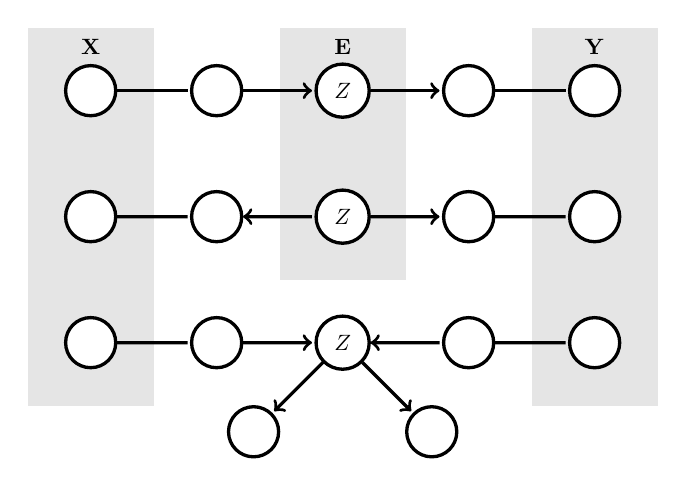
\begin{tikzpicture}[shorten >=1pt,auto,node distance = 2cm, very thick,
                    main node/.style={circle,draw,fill=white,font=\bfseries,inner sep=8pt},pos=0.25,scale=0.8, transform shape]

          \path[fill=gray!20] (-1,-5) -- (-1,1) -- (1,1) -- (1,-5);
          \path[fill=gray!20] (7,-5) -- (7,1) -- (9,1) -- (9,-5);
          \path[fill=gray!20] (3,-3) -- (3,1) -- (5,1) -- (5,-3);

          \draw (0,0.7)   node[] {\textbf{X}};
          \draw (4,0.7)   node[] {\textbf{E}};
          \draw (8,0.7)   node[] {\textbf{Y}};

          \node[main node] (1) []{};
          \node[main node] (2) [right of=1]{};
          \node[main node] (3) [right of=2,inner sep=4.9pt]{$Z$};
          \node[main node] (4) [right of=3]{};
          \node[main node] (5) [right of=4]{};

          \node[main node] (6) [below of=1]{};
          \node[main node] (7) [right of=6]{};
          \node[main node] (8) [right of=7,inner sep=4.9pt]{$Z$};
          \node[main node] (9) [right of=8]{};
          \node[main node] (10) [right of=9]{};

          \node[main node] (11) [below of=6]{};
          \node[main node] (12) [right of=11]{};
          \node[main node] (13) [right of=12,inner sep=4.9pt]{$Z$};
          \node[main node] (14) [right of=13]{};
          \node[main node] (15) [right of=14]{};

          \node[main node] (16) [below left of=13]{};
          \node[main node] (17) [below right of=13]{};



          \path
          (1) edge [] node [] {} (2)
          (2) edge [->] node [] {} (3)
          (3) edge [->] node [] {} (4)
          (4) edge [] node [] {} (5)

          (6) edge [] node [] {} (7)
          (7) edge [<-] node [] {} (8)
          (8) edge [->] node [] {} (9)
          (9) edge [] node [] {} (10)

          (11) edge [] node [] {} (12)
          (12) edge [->] node [] {} (13)
          (13) edge [<-] node [] {} (14)
          (14) edge [] node [] {} (15)

          (13) edge [->] node [] {} (16)
          (13) edge [->] node [] {} (17);


        \end{tikzpicture}
    \end{center}
\end{halfboxr}

\section{Learning}
\subsection{Kinds of Feedback during Learning}

In \emph{supervised learning}, the learner has access to input and correct output.

\emph{Reinforcement learning} only gives feedback in terms of rewards and punishment, but not correct answers.

\emph{Unsupervised learning} happens without any feedback to the learner. The learner must learn on its own.
\vspace{-0.5\baselineskip}
\subsection{Decision Trees}

\begin{halfboxl}
We can measure the average amount of information produced by some stochastic source of data with probabilities using the metric \emph{(information) entropy}.
High entropy means the source generates more information.
For our purposes, low entropy also means the source can be predicted more easily.

Consider a fair coin flip with probabilities $\frac{1}{2}$ for both heads and tails.
This source has entropy $\operatorname I(\frac{1}{2}, \frac{1}{2}) = 1$.
However, a biased coin, e.g.\ one with probability $\frac{99}{100}$ has entropy $\operatorname I (\frac {99}{100},\frac 1 {100}) = 0.08$.
\end{halfboxl}%
\begin{halfboxr}
\vspace{-\baselineskip}
\begin{defi}{Information Entropy}
Let $v_1,\ldots,v_n$ be the outcomes of a probabilistic experiment with probabilities $\operatorname P(v_1),\dots,\operatorname P(v_n)$.
\begin{align*}
\operatorname I(\operatorname P(v_1),&\dots,\operatorname P(v_n)) \\
&:= -\sum\limits_{i=1}^n \operatorname{P} (v_i) \cdot \log_2 (\operatorname{P}(v_i))
\end{align*}

{\footnotesize We define $\log_2 0 := 0$.}
\end{defi}
\end{halfboxr}
\vspace{-0.5\baselineskip}
\begin{defi}{Average Attribute Entropy}
Let $a$ be an attribute with $n$ negative and $p$ positive examples.
Further, let $p_i$ respectively $n_i$ be the number of positive respectively negative occurrences of attribute value $i$.
\[\operatorname{AI} (a) = - \sum\limits_\text{value $i$} \left (\frac{p_i + n_i}{p+n} \cdot \operatorname{I} \left ( \frac{p_i}{p_i+n_i},~ \frac{n_i}{p_i+n_i} \right) \right )\]
\end{defi}

\begin{halfboxl}
\emph{Decision tree-learning} now builds decision trees by choosing attributes with the lowest average entropy until the attribute set only has \texttt{Yes} or \texttt{No} results.

The key idea is that, to build a small decision tree, and assuming the the simplest hypothesis is the most likely, lowest average entropy is a metric of how good an attribute is at predicting the final decision.

{\footnotesize (Most definitions of decision tree-learning use \emph{information gain} instead of average attribute entropy. Our definition simplifies the algorithm by omitting unnecessary constant terms.)}
\end{halfboxl}%
\begin{halfboxr}
\vspace{-\baselineskip}
\begin{algo}{Decision Tree-Learning}
\textbf{Input}: A set of examples with attributes.

\textbf{Output}: A decision tree.
\tcblower
\begin{enumerate}
    \item Choose $a = \argmin_a \operatorname{AI}(a)$, the attribute with the lowest average entropy.
    \item Create a node for $a$:
        \begin{itemize}
            \item If $a$ only has positive or negative examples, return a leaf with \texttt{Yes} or \texttt{No} accordingly.
            \item Otherwise recursively build subtrees for each value with the remaining attributes.
        \end{itemize}
\end{enumerate}
\end{algo}
\end{halfboxr}



\subsection{Neural Networks}

Neural networks are kind of similar to the human brain (but not in any detail).
\emph{Neural networks} consist of \emph{units} (neurons) with \emph{links} (synapses) between units with input and output edges.
These edges have \emph{weights}, usually real numbers.
Units have an output value based on its weighted inputs called \emph{activation level}.
Special \emph{input and output units} are connected to the external environment.

The output $a_i$ of a unit $i$ is usually calculated using some nonlinear function $g$.
\[ a_i := g \left( \sum_j W_{j,i} \cdot a_j \right) \]

\subsubsection{Network Topologies}

\emph{Feed-forward networks} are connected like a directed acyclic graph.
Here, we call units that are not connected to the environment \emph{hidden units}.
Special cases of feed-forward networks are \emph{perceptrons} which do not have hidden units.

\emph{Recurrent networks} have arbitrarily complex connections.

Networks often have a \emph{layer} structure where units of one layer are only connected to nodes of the next layer.

\subsubsection{Neural Network Learning}

The following simple learning algorithm for perceptrons will always converge to the correct output for representable functions.
Unfortunately, perceptrons can only represent linearly separable functions.

\begin{algo}{Perceptron Learning}
\textbf{Input}: Set of $examples$ and learning rate $\alpha$.

\textbf{Output}: A perceptron.
\tcblower
\begin{enumerate}
    \item Initialise $network$ with randomly assigned weights.
    \item Repeat until examples are correctly predicted or stopping criterion is reached:
        \begin{itemize}
            \item For each example $e \in examples$:
                \begin{enumerate}
                    \item Let $I$ be the input for $e$ and $T$ be the actual observed output for $e$.
                    \item Calculate output $O$ using current $network$ and input $e$.
                    \item Update weights: $W_j = W_j + \alpha \cdot I_j \cdot (T - O)$.
                \end{enumerate}
        \end{itemize}
    \item Return $network$.
\end{enumerate}
\end{algo}

The learning algorithm is a bit more complex for multi-layer feed-forward networks.
It is called \emph{back-propagation}, because it propagates updates backwards through the network.

\begin{algo}{Back-Propagation}
\textbf{Input}: Set of $examples$ and learning rate $\alpha$ and base $network$.

\textbf{Output}: A multi-layer feed-forward network.
\tcblower
\begin{enumerate}
    \item Repeat until examples are correctly predicted or stopping criterion is reached:
        \begin{itemize}
            \item For each example $e \in examples$:
                \begin{enumerate}
                    \item Let $I$ be the input for $e$ and $T$ be the actual observed output for $e$.
                    \item Calculate output $O$ using current $network$ and input $e$.
                    \item Compute error in output layer: $Err = T - O$.
                    \item Update weights in output layer: $W_{j,i} = W_{j,i} + \alpha \cdot a_j \cdot (T_i - O_i) \cdot g'(in_i)$.
                    \item For each subsequent layer:
                        \begin{enumerate}
                            \item $\delta_j = g'(in_j) \cdot \sum_i W_{j,i} \delta_i$
                            \item $W_{k,j} = W_{k,j} + \alpha \cdot I_k \cdot (T_i - O_i) \cdot g'(in_i)$.
                        \end{enumerate}
                \end{enumerate}
        \end{itemize}
    \item Return $network$.
\end{enumerate}
\end{algo}

\end{document}
